% !TEX program = xelatex
\documentclass[
  10pt,
  twoside,
  openany,
  b5paper, % 以上均为 ctexbook 提供的文类选项
  colorscheme = basic, % 请根据需要选择或定制配色方案
]{qyxf-book}

\usepackage{graphicx}
\usepackage{epstopdf}
\usepackage[journal=jacs]{chemstyle} 
\usepackage{subcaption}
\usepackage{ccicons}
\usepackage{draftwatermark}
\usepackage{fontawesome5}
\SetWatermarkText{振宇考研}
\SetWatermarkLightness{0.92}
\SetWatermarkScale{0.9}

\title{有机化学}
\subtitle{Organic Chemistry}  % 可选
\author{韩玉玺}
\date{2023 年 3 月 1 日}
\typo{Kimariyb 喵小决}  % 排版人员信息,选填

% 定制元信息
\org{\Large\textit{振宇考研}\\\textsc{CLAUSIUS ZHEN YU KAO YAN}}
\footorg{\textsc{ZHEN YU KAO YAN}}
\cover{
\includegraphics[width=.6\textwidth]{logo.pdf}}
\license{}  % 清空许可证信息

% 调整封面标题大小
\renewcommand{\titlefont}{\Huge\bfseries}
\renewcommand{\subtitlefont}{\LARGE\itshape}

\begin{document}

\maketitle

\chapter*{前言}

本书大胆的使用了\LaTeX 与Chemdraw相结合来编写有机化学资料,使用了\href{https://github.com/qyxf/qyxf-book}{钱院学府}的 \LaTeX 模板,在此特别鸣谢。创新的使用了chemstyle宏包,本人选择了该宏包中的jacs主题作为全书的有机结构风格。下面是使用该宏包在有机化合物绘制的使用:

\begin{scheme}[ht]
	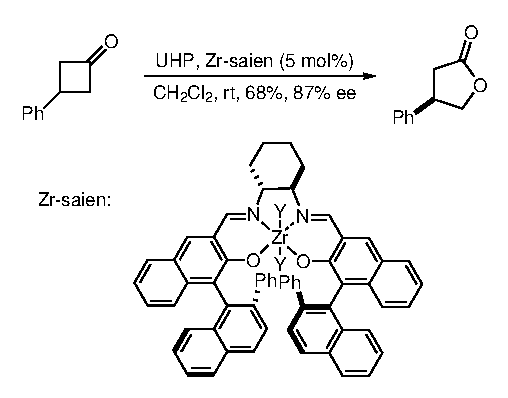
\includegraphics{eg/eg.eps}
	
\end{scheme}

本作品采用\href{https://
	creativecommons.org/licenses/
	by-nc-nd/4.0/}{ BY-
	NC-ND 4.0 协议}进行许可。使用者可以在给出作者署名及资料来源的前提下对本作品进行转载,但不得对本作品进行修改,亦不得基于本作品进行二次创作,不得将本作品运用于商业用途。

如您在参考的过程中发现有任何错误
之处,欢迎您通过下面的方式联系我们,帮助我们改进这份习题:
\begin{itemize}
	\item \faGithub ~~ GitHub平台论坛:\url{https://github.com/kimariyb/organic-chemistry/issues}
	\item \faEnvelopeOpen ~~ 韩老师邮箱:\texttt{1377692745@qq.com}
	\item \faQq ~~ 
	本人QQ:~~\textbf{喵小决}~~2420707848
\end{itemize}

\begin{flushright}
	喵小决\\
	2023 年 3 月 1 日
\end{flushright}

\cleardoublepage

\tableofcontents

\chapter{立体化学}




\end{document}